\documentclass[11pt]{article}
\usepackage[utf8]{inputenc}
\usepackage[T1]{fontenc}
\usepackage{mathptmx}
\usepackage[scaled=.92]{helvet}
\usepackage{courier}
\usepackage{amsmath,amssymb,amsthm,mathtools}
\usepackage{graphicx,subcaption,booktabs,multirow,array,tabularx,longtable}
\usepackage{xcolor,soul,ulem}
\usepackage{pifont}
\usepackage{microtype}
\usepackage{siunitx}
\usepackage{listings}
\usepackage{algorithm2e}
\usepackage{tikz}
\usepackage{pgfplots}\pgfplotsset{compat=1.17}
\usepackage[numbers,sort&compress]{natbib}
\usepackage[colorlinks=true,citecolor=blue]{hyperref}
\usepackage[capitalise]{cleveref}
\usepackage{enumitem}
\usepackage{fancyhdr}\pagestyle{fancy}
\usepackage[margin=1in]{geometry}
\newtheorem{theorem}{Theorem}
\newcommand{\cmark}{\ding{51}}

\title{A Manuscript With Many Packages}
\author{Author One \and Author Two}
\begin{document}
\maketitle
\begin{abstract}
We test a typical manuscript preamble \cite{knuth84}. \cmark\ done.
\end{abstract}
\section{Introduction}\label{sec:intro}
Text with \textcolor{red}{colour}, \hl{highlight}, \SI{3.5}{\meter\per\second}, and \cref{sec:intro}.
\begin{theorem}\label{thm:a} For all $x\in\mathbb{R}$, $\sin^2 x+\cos^2 x=1$. \end{theorem}
\begin{proof} Trivial. \end{proof}
\begin{algorithm}[H]
\KwData{$n$}\KwResult{$s$}
$s \gets 0$\;
\For{$i\gets1$ \KwTo $n$}{$s \gets s+i$\;}
\caption{Sum}
\end{algorithm}
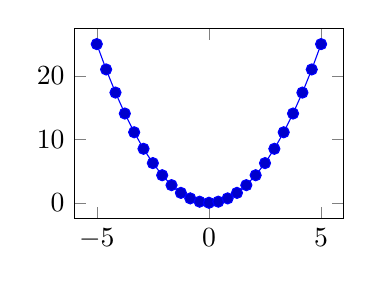
\begin{tikzpicture}
\begin{axis}[width=5cm,height=4cm]\addplot{x^2};\end{axis}
\end{tikzpicture}
\begin{lstlisting}[language=Python]
print("hello")
\end{lstlisting}
\bibliographystyle{plainnat}
\bibliography{refs}
\end{document}
